\documentclass[a4paper]{article}
\usepackage{graphicx}
\usepackage{wrapfig}
\usepackage{float}
\usepackage[rightcaption]{sidecap}
\usepackage[top=1.25in, bottom=1.25in, left=1.25in, right=1.25in]{geometry}
\usepackage[style=authoryear,firstinits=true,backend=bibtex]{biblatex}
\addbibresource{references.bib}
\graphicspath{{images/}}

% Add comma and space after Author name
\renewcommand*{\nameyeardelim}{\addcomma\addspace}

\begin{document}
	
\title{Final year project proposal:\\Implementation of a compiler for Ralang}
\author{Daniel Pacheco\\
	School of Computing and Digital Technology\\
    Faculty of Computing, Engineering and the Built Environment\\
    Birmingham City University\\
	\texttt{Daniel.Pacheco@mail.bcu.ac.uk}}
\date{\today}
\maketitle

\newpage
\tableofcontents

% Show roman numerals in section
\renewcommand{\thesection}{\Roman{section}.}

\newpage
\section{Introduction}
Computer programming is across a range of different subjects such as Computer Science, Biology, Mathematics, Physics, etc. For that reason the first programming language is very important and critical choice to make. When the programming language is too hard students will become overwhelmed with the amount of work they have to do and might give up on the subject whilst if it's too easy then the students will be under qualified for a job after they graduate.

\subsection{Aim}
The aim of this project is to design and implement a compiler for a programming language to assist students currently enrolled in a computer science degree. This language is purely education and is not meant to replace any existing language currently in use, but to compliment them by providing the same functionality in a neater syntax so that students can familiarise themselves with computer programming instead of running into problems caused by syntactically incorrect programs as described by \textcite{KrpanBilobrk2011}.

\subsection{Objectives}
\begin{enumerate}
	\item The syntax of the language should be relatively easy for students taking a programming module in higher education. This can be evaluated by carrying out a simple test along with a questionnaire. Using statistics to compare the results to previous tests, the outcome of the tests can be obtained relatively quick as soon as the questionnaires have been filled in and the tests completed.
	\item Given the amount of time provided to complete this project it's important to only focus on improving the correctness of the program rather the program's efficiency. \textcite{AhoLamSethiUllman2006} says the code optimisation process must also be correct to preserve the meaning of the compiled program, this means focusing more on the code generation will achieve better results.  overall. It will then be possible to execute pre-defined test programs and data to evaluate whether the compiler provides the correct results.
	\item The compiler is able to compile source code both for Linux and Windows operating system. Various number of tests will be used to check if the program performance has a significant changes in both these Operating Systems, or if they perform at the same level. To do this, a virtual machine will be created and given the same amount of memory, then tests can be performed. Setting up virtual machines and writing the test cases may take some time, nevertheless this will allow the creation of statistics on the data obtained from the results to compare the performance of the programming language in different operating systems.
\end{enumerate}

\subsection{Research methodologies}
Only peer-reviewed journals and papers, and books on the compiler writing are going to be used through-out this research. Peer-reviewed journals and papers will be filtered out by skimming through abstracts and introductions, as time is a constraint for this project. The most relevant 10 to 15 journals and papers will be selected for the literature review. Well known books will be referenced in the reference section at the end. Books will only be used if there are no relevant papers on the subject.

\newpage
\section{Literature review}

\subsection{Introduction}
Computer programming is a fundamental requirement at any Bachelor of Science degree such as physics, biology and computer science. Nevertheless, learning a programming language can be a difficult and taunting challenge for people who have not programmed before. \textcite{VihavainenAiraksinenWatson2014} says despite the enormous efforts to improve CS failure rates, these numbers are still very high across the board. Institutions also have to ensure students enrolled in computer programming courses are able to understand the content of the course and at the same time the students must be prepared to use the skills gained to go into industry confident and able to perform the required jobs. \parencite{KrpanBilobrk2011}\\

This literature review attempts to answer two main questions: What do the majority students enrolled on a computer programming course find difficult and how can this problem be tackled. How the problem can be tackled also needs to take into consideration programming languages currently being used in the industry, and whether learning a certain pedagogical language, would enable the students to transit to another industry programming language such as Java, C\# or C++ for example.

\subsection{Introductory programming languages}
There are various different approaches to the problem of what programming languages are better to learn as a introductory language. \textcite{Daly2011} compares using Alice/Java course against a pure Java course. Alice is a object-oriented 3D programming environment used to introduce students to computer programming. The results carried out of this research found that students learning Java along with Alice were a lot more confident than those learning pure Java. Even though \textcite{Daly2011} concludes that students that learn Alice alongside Java seem to be more enthusiastic about taking another programming course than those that learn pure Java, it failed to address the issue of how well the students actually performed in the end in terms of being able to write a simple computer program.\\

\textcite{KrpanBilobrk2011} takes a similar approach to the problem above but this time around students are learning C, QBasic and Python. In this experiment the students attempt 3 different exercises: calculating factorial of n, reversing a string and counting words in a text file. The students seemed more confident about programming in Python, and rated C as the most difficult programming language to use, nevertheless achieved an overall better results in the C language.\\

\begin{wrapfigure}{l}{0.5\textwidth}
	\vspace{-20pt}
	\begin{center}
		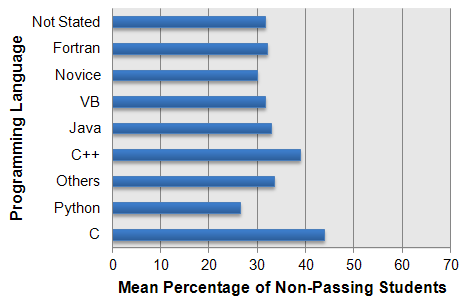
\includegraphics[width=0.48\textwidth]{NonPassingStudents}
	\end{center}
	\caption{Non-passing students grouped by programming language. \parencite{WatsonLi2014}}
	\vspace{-10pt}
\end{wrapfigure}

\textcite{WatsonLi2014} obtained a more comprehensive set of results by combining data from 145 universities and 16 college from various different countries and looking at the top programming languages used at these institutions. Figure 1, compares Fortran, Novice, VB, Java, C++, Python, C and other languages. Python programming language in this case achieves the best mean percentage, whilst C programming language seems to get more non-passing students, nevertheless as mentioned in \textcite{WatsonLi2014}, the mean percentage of non-passing students does not seem to vary extraordinarily as the results range from 25\% to 45\% and remains consistent throughout.\\

In \textcite{WatsonLi2014}, shows that there are trends mean percentage of non-passing students is actually decreasing over the years. This could be due to the fact that easier to learn programming languages are being introduced, and therefore it is easier for students to pass. This does not necessarily mean that students will be able to solve problems by themselves after they finish the computer programming course, and this could be an issue in the future.\\

Another problem is whether the students will be able to tackle issues by themselves when they finish their course. \textcite{JayalLauriaTuckerSwift2011} says that there is a positive increase in the number of students taking Python as their first programming language. It reason that students taking Python can focus more on the problems themselves rather than syntactic issues. This means that students taking Python as their first language are more likely to be able to tackle issues by themselves.\\

Python is getting a lot of popularity in computer programming course as an introductory language. \parencite{Yadin2011} Python programs allow students to focus on the procedural programming allowing them to think of problems and how to solve them using algorithms. Students tend to find object-oriented programming and this could be the reason why Java seems to lower the confidence levels in students when taught as a first programming language like shown in \textcite{Daly2011}. In fact, many institutions were able to lower the drop out rate by introduction Python as an introductory programming language. \parencite{NikulaSajaniemiTedreWray2007}\\

Similar issues apply when teaching functional programming to first years. \textcite{ChakravartyKeller2004} says that functional programming is hardly a good idea for a student who has never came across programming before. 

\subsection{Conclusion}
At various different institutions around the world different approaches are being taken to lower the number of drop out and to increase the number of students who will be motivated enough to pursue another computer programming course. A lot of these institution seem to be preferring a Python approach to this problem, and drop outs seem to be decreasing. \parencite{JayalLauriaTuckerSwift2011}\\

Nevertheless, the trend doesn't seem to be mutual across every institution as the results tends to vary and indicate otherwise as observed by \textcite{KrpanBilobrk2011} where the average students preferred Python but achieved an overall better grade in C. A slight different case where students across 144 different universities obtained about the same performance in different languages, suggesting the language might not impact how well students solve problems using the computer. \parencite{WatsonLi2014}\\

It's also important to note that students learning procedural programming rather than objected-oriented or functional programming, are able to perform better when it comes to writing algorithms and solving problems. \parencite{Kolling1999}

It is also important to note that most of the statistics provided in the above papers were very limited and might not represent fully correct data, as only samples were collected. The largest sample of data found was done to 161 institutions from all around the world.

\newpage
\section{Design}

\subsection{Requirement specification}

Ralang source code should be easy to read and easy to write. By comparing Java source code with Ralang source code in Figure 2. it's clear that Ralang requires less lines of code and less characters to print "Hello, World" to the screen, meaning that student will have to write much less to obtain the same results.\\
\begin{figure}[H]
	\vspace{-10pt}
	\begin{center}
		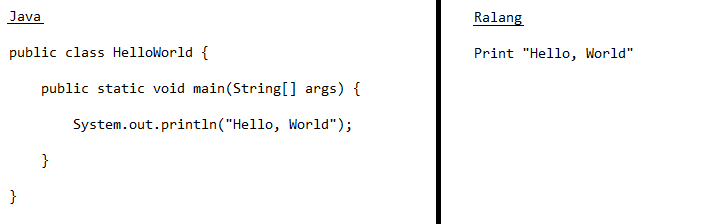
\includegraphics[width=\textwidth]{sampleRalang}
	\end{center}
	\caption{"Hello, World" in Java and Ralang.}
	\vspace{10pt}
\end{figure}
Objective 3 for this project is that the compiler for Ralang must be able to run both on Windows and Linux operating system. In order to make that happen the source code of the program is compiled to Java bytecode to run on the Java Virtual Machine. There are several languages that will run on the JVM such as Java, Scala, Clojure and Jython. A functional programming would be more suitable for this project because of compiler work a lot with trees and also pattern matching, in which case Clojure may be very suitable.\\

To understand whether the programming language meets the requirements, a simple test along with a questionnaire will be carried out to first and second year students, who may have prior programming knowledge and they will be required to follow a written or video tutorial, then write a simple application and finally answer some questionnaire questions about how they feel about the language.\\

\textcite{AhoLamSethiUllman2006} lays out the seven different phases to writing a compiler: Lexical, syntax and semantic analyser, intermediate code generator, machine-independent code optimiser, code generator and machine-dependent code optimizer. To ensure the project can be successfully completed within a certain time frame, code optimisation will be skipped. In that case more time can be spent to ensure the correctness of the compiler.\\

From the literature review, it was concluded that the Python programming language is used to at various institutions to introduce students to computer programming, nevertheless many students claimed Python was far easier than languages like C but still the overall average performed better in C. \parencite{KrpanBilobrk2011}\\

It was understood the majority of people preferred Python because of its neat and clear syntax but due to being a dynamic programming language students tend to have many problem being able to write and run their own programs.

Ralang will implement static typing, where the compiler will do various checks and report errors where possible but also implement a neat and clear syntax like Python.

\subsection{Development methodologies}
There are several development methodologies available to use for this project such as Rapid Application Development (RAD) or scrum software development.\\

Scrum software development assumes that the problem can not be completely laid out, and changes may be made along the way. This methodology allows quick prototyping and would allow quick deliverables, so it would work well for projects that would require to be changed frequently.

Similarly, RAD provides a fast development process and it's easy to adjust to the requirements of the project. It will allow easy prototyping and making changes as necessary to obtain best results possible, whether that would be the correctness of the program, or changes to the syntax of language or even how to deal with compiling errors.\\

RAD seems the most suitable methodology as the development of the project won't be altering constantly, there might be slight changes along the way until the final product is complete, nevertheless the changes will always be minor until the end product is finished.

\newpage
\printbibliography

\end{document}